\documentclass[12pt, letterpaper]{../assignment}
\usepackage{graphicx}
\usepackage{courier}
\usepackage{minted}
\usepackage{amsmath}
\usepackage{commath}
\usepackage{amssymb}
\usepackage{amsfonts} 
\usepackage{cancel}
\usepackage{enumitem}
\usepackage{array}

\usepackage{tikz}
\usetikzlibrary{shapes,arrows,positioning}

\usemintedstyle{monokai}
\oddsidemargin = 0pt
\exercisesheet{Module 8}{Practice Assignment}
\student{Austin Barrilleaux}
\courselabel{EN 525.609}
\semester{Fall 2023}
\usepackage[backend=bibtex,style=numeric,sorting=none]{biblatex}
\bibliography{reference}
\usepackage{color}
\definecolor{light-gray}{rgb}{0.2,0.2,0.2}
\setminted{bgcolor=light-gray}
\setlength{\parindent}{0pt}

\makeatletter
\patchcmd{\minted@colorbg}{\noindent}{\medskip\noindent}{}{}
\apptocmd{\endminted@colorbg}{\par\medskip}{}{}
\makeatother

\begin{document}
\subsection*{Problem 1}
\subsubsection*{Solve the following practice problems in the 9th edition textbook.\\
\begin{itemize}
    \item Chapter 5:
    \begin{itemize}
        \item 7-1 (a)
        \item 7-6 (a)
    \end{itemize}
\end{itemize}}

\subsubsection*{7-1. Find the angles of the asymptotes and the intersect of the asymptotes of the root loci of the following equations when $K$ varies from $-\infty$ to $\infty$.}

\subsubsection*{(a) \ \  $ \mathbf{s^4 + 4s^3 + 4 s^2+ (K+8)s + K = 0}$}

Putting the above equation into the form:

$$ 1 + \frac{K Q(s)}{P(s)} = 0 $$

We get:

$$ Q(s) = s + 1  $$

And:

$$ P(s) = s^4 + 4s^3 + 4 s^2+ 8s $$


The poles are, (using the \texttt{roots()} function in MATLAB):

$$ \texttt{roots([1,4,4,8,0])} = \left[ \begin{array}{cc} 
    \ \ 0.0000 &+ 0.0000j\\
    -3.5098 &+ 0.0000j\\
    -0.2451 &+ 1.4897j\\
    -0.2451 &- 1.4897j
\end{array} \right] $$

The zero is $s = -1$.
\\\\
Factoring $P(s)$ results in $4$ poles, and the equation has $1$ zero:
\\\\
For large values of $s$, the root locus for $K > 0$ are asymptotic to asymptotes with angles
given by:

$$ \theta_i = \frac{(2i+1)}{|n-m|} \times 180^{\circ}, \ \ n \neq m, \ \ i = 0,1,2... \ |n-m|-1$$

For this case:

$$ |n-m|-1 = |4-1|-1 = 2 \rightarrow i = 0,1,2 $$

Therefore, when $K > 0$ :

\begin{answer}
    $$ \theta_0 = \frac{(2(0)+1)}{3} \times 180^{\circ} = 60^{\circ}, \ \ [K > 0] $$
\end{answer}

\begin{answer}
    $$ \theta_1 = \frac{(2(1)+1)}{3} \times 180^{\circ} = 180^{\circ}, \ \ [K > 0] $$
\end{answer}

\begin{answer}
    $$ \theta_2 = \frac{(2(2)+1)}{3} \times 180^{\circ} = 300^{\circ}, \ \ [K > 0] $$
\end{answer}

For large values of $s$, the root locus for $K < 0$ are asymptotic to asymptotes with angles
given by:

$$ \theta_i = \frac{(2i)}{|n-m|} \times 180^{\circ}, \ \ n \neq m, \ \ i = 0,1,2... \ |n-m|-1$$

Where again:

$$ |n-m|-1 = |4-1|-1 = 2 \rightarrow i = 0,1,2 $$

Therefore, when $K < 0$ :

\begin{answer}
    $$ \theta_0 = \frac{(2(0))}{3} \times 180^{\circ} = 0^{\circ}, \ \ [K < 0] $$
\end{answer}

\begin{answer}
    $$ \theta_1 = \frac{(2(1))}{3} \times 180^{\circ} = 120^{\circ}, \ \ [K < 0] $$
\end{answer}

\begin{answer}
    $$ \theta_2 = \frac{(2(2))}{3} \times 180^{\circ} = 240^{\circ}, \ \ [K < 0] $$
\end{answer}

The point of intersection of the asymptotes is given by:

$$ \sigma_1 = \frac{\sum \text{real parts of poles of } G(s)H(s) - \sum \text{real parts of zeros of } G(s)H(s) }{n-m} $$

Where:

$$ G(s)H(s) = \frac{K Q(s)}{P(s)} $$

Evaluating the sum of the real parts of the poles in MATLAB:

$$ \texttt{sum(real(roots([1,4,4,8,0])))} = -4 $$

Therefore:

\begin{answer}
$$ \sigma_1 = \frac{(-4)-(-1) }{4-1} = -1 $$
\end{answer}

\subsubsection*{7-6. For the loop transfer functions that follow, find the angle of departure or arrival of the root loci at the designated pole or zero.}
\subsubsection*{(a) \ \  $ \mathbf{G(s)H(s) = \dfrac{K s}{(s+1)(s^2+1)}}$}
\subsubsection*{ \ \ \ \ \ \ Angle of arrival $\mathbf{(K < 0)}$ and angle of departure $ \mathbf{(K > 0)}$ at $ \mathbf{s = j}$.}

This equation can be rewritten as:

$$ G(s)H(s) = \dfrac{K s}{(s+1)(s+j)(s-j)} $$



% \color{white}
% \hspace*{6em}\inputminted[frame=leftline,fontsize=\footnotesize]{matlab}
% {./matlab/Problem_5_18.m}
% \color{black}

% \begin{figure}[H]
%     \centering
%     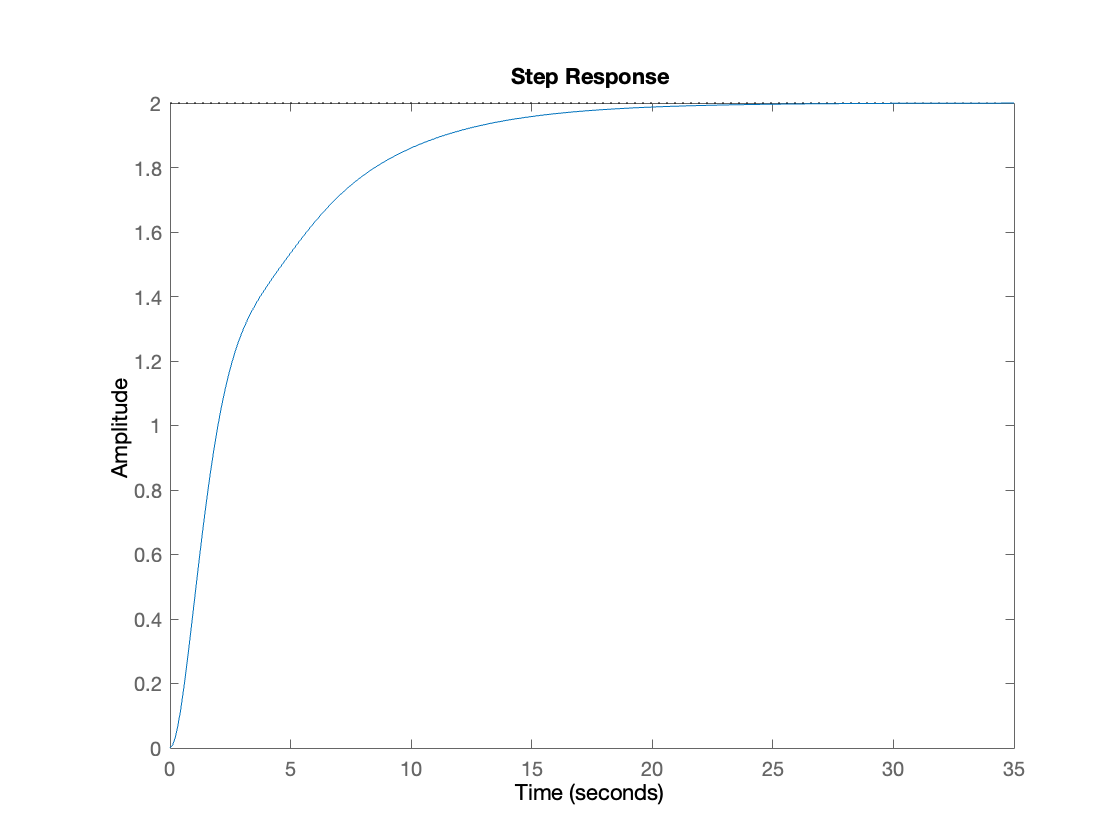
\includegraphics[width=0.7\linewidth]{./figures/step_response.png}
%     \caption{Step Response}
%     \label{fig:step}
%  \end{figure}



\end{document}

